%% Transportation Research Part E submission draft (Elsevier elsarticle, author-year).
%% Overleaf compiler: pdfLaTeX. Red [TODO: ...] marks text or results that do not exist yet.
%% Draft of 2026-11-02. Numbers come from outputs/ in the code repository; see the
%% comment above each table for its source.

\documentclass[preprint,review,12pt,authoryear]{elsarticle}
%% Journal-like layout while drafting: \documentclass[final,3p,times,authoryear]{elsarticle}

\usepackage{amssymb,amsmath,amsthm}
\usepackage{booktabs,multirow}
\usepackage{algorithm,algpseudocode}
\usepackage{graphicx,xcolor}
\usepackage{tikz}
\usetikzlibrary{arrows.meta,positioning,fit}
\usepackage[hidelinks]{hyperref}
\usepackage{lineno}
\linenumbers

\newcommand{\todo}[1]{\textcolor{red}{[TODO: #1]}}
\newtheorem{proposition}{Proposition}
\newtheorem{remark}{Remark}
\newcommand{\R}{\mathbb{R}}
\newcommand{\UB}{\mathrm{UB}}

\journal{Transportation Research Part E: Logistics and Transportation Review}

\begin{document}

\begin{frontmatter}

\title{Learning to route a carrier--drone system from sparse exact feedback:
a self-improving deep reinforcement learning approach}

\author[a]{Jianing Wang\corref{cor1}}
\ead{jianingwang672@gmail.com}
\author[a]{Co-author Name}
\cortext[cor1]{Corresponding author.}
\affiliation[a]{organization={Department, University},
            city={City},
            country={Country}}
%% TODO: co-authors and affiliation

\begin{abstract}
In carrier--drone operations a slow carrier launches a fast drone that visits one target per sortie and
lands on the moving carrier again. The carrier--vehicle traveling salesman problem
(CVTSP) couples a combinatorial visiting order with a second-order cone program (SOCP) that places every
take-off and landing point, so evaluating each order needs one exact SOCP solve. Deep reinforcement learning
(DRL) policies trained with exact SOCP rewards plan in under a second, but training
consumes hundreds of millions of SOCP solves. We propose a self-improving DRL framework that learns from
sparse exact feedback. For each training instance only about three orders are solved exactly. The primal
solution of one solve is converted into a directed cost table that gives a certified upper bound on the
makespan of every other order. Local search on this table produces improved routes without further solves,
and these routes are distilled into the policy by imitation learning while the policy gradient uses the same
bounds as dense rewards. Compared with a POMO policy trained on exact rewards for 200 epochs, the proposed
method uses 15 times fewer training instances and 78 times fewer SOCP solves, at the same inference cost.
It is within 0.12\% of that policy on 529 literature instances, better by 1.26\% on the 200-target instances,
and within 1.05\% on synthetic instances with 20--100 targets. At an equal number of solves, exact-reward
training is 4.2\% worse, and a full mixed-integer SOCP model finds no feasible solution within one hour
for 100 or more targets.
\todo{one sentence of managerial insight once the sensitivity analysis is done.}
\end{abstract}

\begin{highlights}
%% Elsevier highlights: 3--5 bullets, at most 85 characters each (including spaces).
\item A self-improving deep reinforcement learning method for the carrier--vehicle TSP
\item Sparse exact SOCP solves yield certified bounds that score every other route
\item Bound-guided local search creates expert routes for imitation without solves
\item Matches an exact-reward policy with 78 times fewer solves at equal test time
\item Exact MISOCP finds no feasible solution within 1 h for 100 or more targets
\end{highlights}

\begin{keyword}
Carrier--vehicle traveling salesman problem \sep Drone routing \sep Deep reinforcement learning \sep
Second-order cone programming \sep Self-improvement \sep Imitation learning
\end{keyword}

\end{frontmatter}

%% ===================================================================
\section{Introduction}\label{sec:intro}

Drones extend the reach of a vehicle that cannot itself approach every point of interest. A patrol vessel
inspects offshore platforms, buoys or ships with a drone launched from its deck; a relief truck on a damaged
road network sends a drone to isolated sites; a parcel van releases a drone for the last few hundred metres.
In each case a slow carrier moves continuously while a fast drone with limited endurance leaves it, serves one
target and lands on it again at a later position. The carrier--vehicle traveling salesman problem
\citep[CVTSP;][]{garone2010cooperative,gambella2018exact} asks for the visiting order and for the take-off
and landing points that minimise the time until the carrier returns to its depot with all targets visited.
Closely related variants are known as the mothership and drone routing problem \citep{poikonen2020mothership}
and belong to the wider family of drone-assisted routing problems
\citep{murray2015flying,agatz2018optimization,otto2018optimization,macrina2020drone,chung2020optimization}.

The CVTSP is hard for two reasons that compound each other. First, it contains a traveling salesman problem
over the targets. Second, the cost of a given visiting order is not a sum of fixed edge costs: the
take-off and landing points are continuous decisions shared by consecutive sorties, and evaluating one order
requires solving a second-order cone program (SOCP). Exact methods based on mixed-integer SOCP (MISOCP)
formulations, branch-and-bound over orders, or logic-based Benders decomposition
\citep{gambella2018exact,erdogan2021exact,li2025exact} prove optimality for instances with up to about
20 targets; for larger instances the best results come from heuristics that solve many SOCPs per instance
\citep{poikonen2020mothership,li2025exact}.

Deep reinforcement learning (DRL) offers an attractive alternative for repeated operational planning: a
policy network trained offline constructs a good order in milliseconds, and a few exact SOCP solves at test time
turn the order into an executable plan. Attention-based policies trained with policy gradients
\citep{kool2019attention}, in particular POMO \citep{kwon2020pomo}, are now standard for routing problems
whose route cost is a sum of edge costs. For the CVTSP, however, the reward of each sampled route is the
optimal value of an SOCP. A POMO policy trained with exact Gurobi rewards for 200 epochs, which we use as the
main reference (G200), consumed $3.0\times10^{8}$ SOCP solves and about nine days of wall time on 128 solver
workers. The training cost, not the inference cost, is the bottleneck. This cost recurs whenever the
operating conditions change, for example the vessel speed, the drone model or the target geography.

This paper asks whether a CVTSP policy of comparable quality can be trained from \emph{sparse} exact
feedback, that is, from a few exact SOCP solves per training instance instead of one per sampled route. We
answer it with a self-improving DRL framework built on three observations. (i) The primal solution of one
SOCP, relabelled by target, remains feasible for every other visiting order once the carrier transfer legs
are recomputed; this yields a directed $(n+1)\times(n+1)$ cost table whose route sums are certified upper
bounds on the makespan of every order (Proposition~\ref{prop:ub}). (ii) Because the bound is a route sum, local
search moves can be scored in constant time, so a strong improved route (an \emph{expert}) can be found
without solving any further SOCP. (iii) The policy can then learn from two signals at once: imitation of the
expert route, and policy gradients on dense certified-bound rewards anchored by one exact reward per instance.

The contributions are as follows.
\begin{enumerate}
\item We derive certified upper-bound tables for the CVTSP from a single exact SOCP solution and show how
they replace exact evaluation inside both the reward and the local search of a learning algorithm, while every
route that enters the training signal as ``improved'' is verified by an exact solve.
\item We propose a self-improving training framework that combines POMO policy gradients on hybrid
exact/bound rewards, imitation of bound-guided local-search experts, near-miss validation and table
refreshes, and a progressive search schedule that strengthens the expert only where the policy needs it.
The framework uses on average 2.9 exact solves per training instance.
\item In extensive experiments on synthetic instances with 20--500 targets and on the 529 literature
instances of \citet{li2025exact}, the trained policy approaches the quality of a policy trained with exact
rewards on every route while using 15 times fewer instances and 78 times fewer exact solves, with identical
inference cost. At equal solve budget, exact-reward training is clearly worse, and an exact MISOCP model fails
to find feasible solutions for 100 or more targets within one hour.
\item \todo{Managerial contribution: how the speed ratio, endurance and target geography affect makespan,
drone utilisation and the value of a learned planner (Section~\ref{sec:managerial}).}
\end{enumerate}

Section~\ref{sec:lit} reviews related work. Section~\ref{sec:problem} defines the problem and derives the
upper-bound tables. Section~\ref{sec:method} presents the learning framework. Section~\ref{sec:exp} reports the
computational study, Section~\ref{sec:managerial} discusses managerial implications, and
Section~\ref{sec:conc} concludes.

%% ===================================================================
\section{Literature review}\label{sec:lit}

\subsection{Carrier--vehicle and mothership--drone routing}
\citet{garone2010cooperative} introduced the carrier--vehicle problem in which a carrier transports a
short-range vehicle between points of interest. \citet{gambella2018exact} formulated the CVTSP as an MISOCP
and solved instances with up to about 15 targets to optimality; they also proposed a heuristic that
fixes the visiting order and solves the remaining SOCP. \citet{erdogan2021exact} strengthened the
formulation, developed a branch-and-bound algorithm over orders and heuristics for instances with up to 50 targets.
\citet{poikonen2020mothership} studied the closely related mothership and drone routing problem and
generated instances with up to 200 targets on regular and clustered layouts.
Most recently, \citet{li2025exact} proposed an improved MISOCP (Model+), a logic-based Benders decomposition
and a two-stage iterative heuristic (TSIH), and compiled the 529 instances of
\citet{gambella2018exact}, \citet{erdogan2021exact} and \citet{poikonen2020mothership} into a common benchmark
with best-known solutions. A common thread is that the visiting order is the hard part, while the
continuous placement for a fixed order is an SOCP \citep{lobo1998applications} that commercial solvers handle
in milliseconds. Every method therefore spends most of its time in repeated SOCP evaluations.
The CVTSP differs from truck--drone problems such as the flying sidekick TSP
\citep{murray2015flying,agatz2018optimization}, in which launch and recovery happen at customer nodes; see
\citet{otto2018optimization}, \citet{macrina2020drone} and \citet{chung2020optimization} for reviews.

\subsection{Learning-based methods for routing}
Learning-based construction heuristics generate a route node by node with a neural policy
\citep{vinyals2015pointer,nazari2018reinforcement,kool2019attention}. POMO \citep{kwon2020pomo} decodes one
route from every start node and uses their mean reward as a shared baseline for REINFORCE
\citep{williams1992simple}; with geometric augmentation it is a standard benchmark. Sym-NCO
\citep{kim2022symnco} exploits symmetries further, and efficient active search
\citep{hottung2022efficient} adapts a subset of parameters at test time. Improvement-type policies learn
local-search operators \citep{wu2022learning}. All of these methods assume that the cost of a complete route is
cheap to compute, so millions of sampled routes can be scored per epoch. Surveys are given by
\citet{bengio2021machine} and \citet{mazyavkina2021reinforcement}.

Self-improvement replaces or complements policy gradients with imitation of the best solutions the current
policy and a search procedure can find. \citet{luo2023neural} train a heavy-decoder model in a
supervised and then self-improving manner, and \citet{pirnay2024self} sample batches of solutions without
replacement and imitate the best. In these works an improved solution can be recognised because its cost is
cheap to compute. In the CVTSP every comparison between two routes requires two SOCP solves. A search that
evaluates thousands of moves per instance, as these methods do, is therefore impractical.

\subsection{Research gap}
Existing exact and heuristic CVTSP methods solve each instance from scratch with many SOCP evaluations.
Existing learning methods require an exact reward for every sampled route, which for the CVTSP makes training
cost the bottleneck. To the best of our knowledge, no method exploits the structure of the SOCP to
\emph{share} one exact solution across many routes during learning. This paper fills that gap with certified
bound tables, and shows that they support both a dense reward and a solve-free expert search.

%% ===================================================================
\section{Problem description}\label{sec:problem}

\subsection{The CVTSP for a fixed visiting order}
A carrier with speed $V_c$ starts and ends at the depot $p_0\in\R^2$. A drone with speed $V_v>V_c$ and
endurance $a$ must visit targets $p_1,\dots,p_n\in\R^2$, one target per sortie. In sortie $k$ the drone takes
off from the carrier at point $s_k$, flies to target $p_{\pi(k)}$ in time $t^{\mathrm{out}}_k$, returns in
time $t^{\mathrm{in}}_k$ and lands on the carrier at point $l_k$; meanwhile the carrier travels from $s_k$ to
$l_k$. Between sorties the carrier travels from $l_{k-1}$ to $s_k$ in time $T_k$ (with $l_0=p_0$), and finally
back to the depot. For a visiting order (permutation) $\pi$ the minimum makespan $f(\pi)$ is the optimal value of
the SOCP
\begin{align}
f(\pi)=\min\ & \sum_{k=1}^{n} \tau_k + \sum_{k=1}^{n+1} T_k \label{eq:obj}\\
\text{s.t.}\ & \tau_k = t^{\mathrm{out}}_k + t^{\mathrm{in}}_k \le a, && k=1,\dots,n, \label{eq:end}\\
& \|s_k - p_{\pi(k)}\| \le V_v\, t^{\mathrm{out}}_k,\quad \|l_k - p_{\pi(k)}\| \le V_v\, t^{\mathrm{in}}_k,
 && k=1,\dots,n, \label{eq:drone}\\
& \|l_k - s_k\| \le V_c\, \tau_k, && k=1,\dots,n, \label{eq:sync}\\
& \|s_k - l_{k-1}\| \le V_c\, T_k, && k=1,\dots,n, \label{eq:carrier}\\
& \|p_0 - l_n\| \le V_c\, T_{n+1}, \notag
\end{align}
with variables $s_k,l_k\in\R^2$ and $t^{\mathrm{out}}_k,t^{\mathrm{in}}_k,\tau_k,T_k\ge0$.
Constraint \eqref{eq:end} is the endurance limit, \eqref{eq:drone} the drone legs, \eqref{eq:sync} the
synchronisation of drone and carrier during a sortie, and \eqref{eq:carrier} the carrier legs between
sorties. The CVTSP is $\min_\pi f(\pi)$. Since every constraint is a second-order cone, $f(\pi)$ is computed
exactly by an interior-point method; we use Gurobi with the norms written as explicit convex quadratic
constraints. Reversing the order does not change the makespan, $f(\pi)=f(\pi^{\mathrm{rev}})$.
Table~\ref{tab:notation} summarises the notation. \todo{figure: one sortie with $s_k$, $p_{\pi(k)}$, $l_k$.}

\begin{table}[t]\centering\small
\caption{Notation.}\label{tab:notation}
\begin{tabular}{ll}
\toprule
Symbol & Meaning \\
\midrule
$n$ (also $J$) & number of targets \\
$p_0,\ p_j$ & depot, target $j$ \\
$V_c,\ V_v,\ a$ & carrier speed, drone speed, drone endurance \\
$\pi$ & visiting order (permutation of $\{1,\dots,n\}$) \\
$f(\pi)$ & minimum makespan of order $\pi$, SOCP \eqref{eq:obj}--\eqref{eq:carrier} \\
$C^{q}$ & directed upper-bound table built from the exact solution of order $q$ \\
$\UB_q(\pi)$ & certified upper bound on $f(\pi)$ from table $C^q$ \\
$\theta$ & policy parameters \\
\bottomrule
\end{tabular}
\end{table}

\subsection{Certified upper-bound tables}\label{sec:ubtable}
Let $q$ be an order and let $(s^*,l^*,t^{\mathrm{out}*},t^{\mathrm{in}*},\tau^*)$ be an optimal solution of
the SOCP for $q$. Relabel the sortie variables by target: for target $j=q(k)$ write $\hat s_j=s^*_k$,
$\hat l_j=l^*_k$ and $\hat\tau_j=\tau^*_k$. Define the directed table $C^q\in\R^{(n+1)\times(n+1)}$ with
\begin{equation}\label{eq:table}
C^q_{0j}=\frac{\|\hat s_j-p_0\|}{V_c},\qquad
C^q_{ij}=\hat\tau_i+\frac{\|\hat s_j-\hat l_i\|}{V_c},\qquad
C^q_{i0}=\hat\tau_i+\frac{\|p_0-\hat l_i\|}{V_c},
\end{equation}
for $i,j\in\{1,\dots,n\}$, $i\ne j$,
and for any order $\pi$ the route sum
$\UB_q(\pi)=C^q_{0\pi(1)}+\sum_{k=1}^{n-1}C^q_{\pi(k)\pi(k+1)}+C^q_{\pi(n)0}$.

\begin{proposition}\label{prop:ub}
For every order $\pi$, $f(\pi)\le \UB_q(\pi)$, and $f(q)=\UB_q(q)$.
\end{proposition}
\begin{proof}
Assign to sortie $k$ of $\pi$ the relabelled values of target $\pi(k)$: $s_k=\hat s_{\pi(k)}$,
$l_k=\hat l_{\pi(k)}$, and the corresponding drone times. Constraints \eqref{eq:end}--\eqref{eq:sync} involve
only the variables of one sortie and its own target, so they hold because they held for $q$. Set
$T_k=\|s_k-l_{k-1}\|/V_c$ and $T_{n+1}=\|p_0-l_n\|/V_c$; then \eqref{eq:carrier} holds with equality. The
solution is feasible for the SOCP of $\pi$ and its objective equals $\UB_q(\pi)$, hence
$f(\pi)\le\UB_q(\pi)$. For $\pi=q$ the carrier legs of an optimal solution are tight, so the objective equals
$f(q)$.
\end{proof}

The table is asymmetric, since $\hat s_j\neq\hat l_j$ in general. It is tight at the anchor $q$ and loose for
orders that would move the take-off and landing points far from their anchor positions. A move that changes
a few adjacencies, such as 2-opt, changes $\UB_q$ by a few table entries, so it can be evaluated in constant
time.\footnote{For a directed table a 2-opt move reverses a segment, and all directed edges inside the segment
change; the implementation computes these deltas incrementally with prefix sums.} The minimum of
several tables, $\min_m \UB_{q_m}(\pi)$, is again a certified bound. In contrast, the entry-wise minimum of two
tables is not, because it splices two different primal solutions.

%% ===================================================================
\section{Self-improving learning framework}\label{sec:method}

\subsection{Overview}
Figure~\ref{fig:framework} shows one training step for a batch of instances. A frozen \emph{reference} policy
proposes candidate orders, one of which is solved exactly (the \emph{anchor}). Its table $C^{\text{anchor}}$
scores all candidates, and fixed-table local search improves the best and most diverse ones without any solve.
The best resulting order (the \emph{expert}) is verified by one exact solve if it differs from the anchor.
The trainable \emph{target} policy is updated twice: by a policy gradient on rewards that combine one exact
makespan with certified bounds for all other routes, and by imitation (teacher-forced cross-entropy) of the
verified experts. The reference policy is replaced by the target policy only when the target is strictly better on a
fixed validation set. Algorithm~\ref{alg:train} gives the details.

\begin{figure}[t]\centering
\resizebox{\textwidth}{!}{%
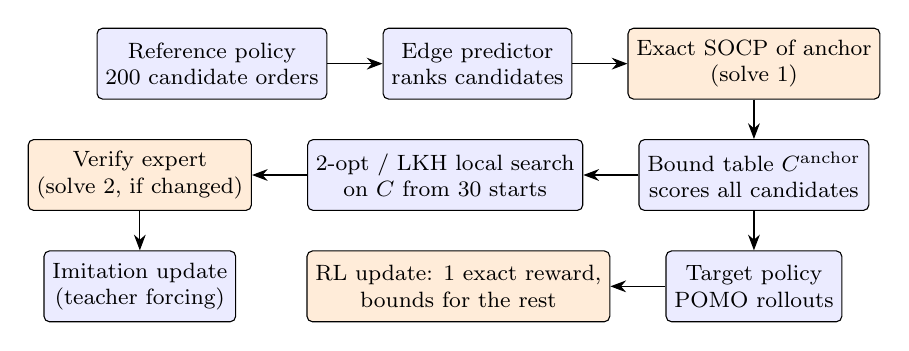
\begin{tikzpicture}[node distance=5mm and 7mm, >={Stealth[length=2mm]},
  box/.style={draw, rounded corners=2pt, align=center, font=\footnotesize, minimum height=9mm, inner sep=3pt},
  exact/.style={box, fill=orange!15}, free/.style={box, fill=blue!8}]
\node[free] (ref) {Reference policy\\200 candidate orders};
\node[free, right=of ref] (pred) {Edge predictor\\ranks candidates};
\node[exact, right=of pred] (anc) {Exact SOCP of anchor\\(solve 1)};
\node[free, below=of anc] (tab) {Bound table $C^{\text{anchor}}$\\scores all candidates};
\node[free, left=of tab] (ls) {2-opt / LKH local search\\on $C$ from 30 starts};
\node[exact, left=of ls] (exp) {Verify expert\\(solve 2, if changed)};
\node[free, below=of exp] (il) {Imitation update\\(teacher forcing)};
\node[free, below=of tab] (tgt) {Target policy\\POMO rollouts};
\node[exact, left=of tgt] (rl) {RL update: 1 exact reward,\\bounds for the rest};
\draw[->] (ref) -- (pred); \draw[->] (pred) -- (anc); \draw[->] (anc) -- (tab);
\draw[->] (tab) -- (ls); \draw[->] (ls) -- (exp); \draw[->] (exp) -- (il);
\draw[->] (tgt) -- (rl); \draw[->] (tab) -- (tgt);
\end{tikzpicture}}
\caption{One training step for one instance. Orange boxes call the exact SOCP solver; blue boxes are
solve-free. \todo{redraw as a polished figure.}}\label{fig:framework}
\end{figure}

\subsection{Policy network and POMO decoding}
The policy is the attention encoder--decoder of \citet{kool2019attention} trained in the POMO manner
\citep{kwon2020pomo}. Each target is embedded from its position relative to the depot, normalised by the
largest target distance, together with instance-level features: the speed ratio $V_c/V_v$ and the normalised
drone reach $V_v a$. The encoder has four layers of 16-head self-attention with embedding dimension 256 and
feed-forward dimension 512 \citep{vaswani2017attention}. The decoder selects the next target with a
single-head pointer attention whose logits are clipped at 10, masking visited targets. At test time the
policy decodes greedily from $\min(n,100)$ start targets (the ones nearest the depot) on each of eight geometric
views of the instance (rotations and reflections), every distinct order is solved exactly, and the best
makespan is returned.

\subsection{Anchor selection, bound scoring and expert search}\label{sec:expert}
For each training instance the frozen reference policy samples 200 candidate orders. A lightweight directed
edge predictor, trained on the tables of earlier batches with a Huber loss, ranks them and selects the anchor
to be solved exactly (solve~1). The anchor's table $C^{\text{anchor}}$ then scores all candidates exactly in
the sense of Proposition~\ref{prop:ub}.

Local search starts from 30 candidates: the 20 with the lowest bound and 10 chosen for diversity from the next
60, provided their bound is within 5\% of the best. From each start we run first-improvement 2-opt on
$C^{\text{anchor}}$ for at most 30 accepted moves, accepting only a strict decrease of the bound. Because
$\UB_{\text{anchor}}(\text{anchor})=f(\text{anchor})$, any route whose bound is below the anchor's exact makespan is
certified to be strictly better than the anchor. The route with the lowest bound becomes the expert. If it
differs from the anchor, it is solved exactly (solve~2), so the expert label always carries its exact
makespan, and its own table $C^{\text{expert}}$ becomes available.

Two mechanisms recover improvements that a single loose table misses. \emph{Near-miss validation}: when no
route certifies an improvement, the best non-anchor route is solved exactly with a probability between 1\% and
5\% that adapts to the policy's imitation accuracy, and it is accepted if its exact makespan beats the anchor.
\emph{Table refresh}: for large instances later in training (Section~\ref{sec:recipe}), the search is repeated
on the table of the latest solved route, which is tight in a different region of the order space, and the best
unsolved result is solved and accepted only if it is exactly better.

\subsection{Hybrid reinforcement and imitation updates}
The target policy samples $P$ POMO rollouts $\pi^{1},\dots,\pi^{P}$ per instance. Their costs are
\begin{equation}
c^{p}=\min\{\UB_{\text{anchor}}(\pi^{p}),\ \UB_{\text{expert}}(\pi^{p})\},\qquad p=1,\dots,P,
\end{equation}
except for one selected rollout whose cost is its exact makespan (one more solve). Advantages are centred by
the POMO mean and standardised within the instance,
$A^{p}=-(c^{p}-\bar c)/\max(\sigma_c,\epsilon)$, and the policy loss is the REINFORCE estimate
$\mathcal L_{\mathrm{RL}}=-\frac{1}{BP}\sum_{b,p}A^{p}_b\log p_\theta(\pi^{p}_b)$. An auxiliary term rewards the
exactly solved rollout relative to the exact expert makespan, clipped to $[-1,1]$ in relative terms; its weight
rises from 0 to 1 as the imitation accuracy of the previous epoch grows from 0.50 to 0.85.

The imitation update is a separate optimiser step on the teacher-forced cross-entropy of verified expert
routes,
$\mathcal L_{\mathrm{IL}}=-\frac{1}{n}\sum_{t=1}^{n}\log p_\theta(e_t\mid e_1,\dots,e_{t-1})$,
for five inner passes over a buffer that mixes the current batch with 30\% replayed experts from a buffer of
50{,}000. Experts that improve on the anchor are up-weighted so that the imitation mass per instance stays
near a fixed target (1.44 samples per instance) as the improvement rate changes.

\subsection{Progressive search schedule}\label{sec:recipe}
Early in training the policy is weak and almost any 2-opt search improves it; later the policy itself proposes
2-opt-optimal routes and the expert stops improving, mostly for large instances. Stronger search everywhere,
however, collapses the diversity of the POMO rollouts for small instances. We therefore strengthen the
expert only for $n\ge60$ and only gradually. With the ramp $r=\mathrm{clip}((\text{epoch}-40)/60,0,1)$, a
fraction $0.5\,r$ of the local-search starts uses LKH-3 \citep{helsgaun2017lkh3} on the bound table instead of
2-opt, the near-miss probability rises to $\text{rate}+r(1-\text{rate})$ (100\% from epoch 100), and two
table-refresh rounds are run from epoch 61. Instances with $n<60$ keep plain 2-opt and adaptive near-miss
validation throughout.

\subsection{Exact-solve accounting}
Per instance, training uses one solve for the anchor, one for the exactly rewarded rollout, at most one for
the expert or near-miss route, and, for large instances late in training, one per refresh round. The number of
solves does not depend on the number of POMO rollouts or local-search moves. Over the whole run the average is
2.89 solves per training instance (Table~\ref{tab:budget}). In contrast, exact-reward training solves every
distinct sampled route.

\begin{algorithm}[t]
\caption{Self-improving training (one batch $\mathcal B$)}\label{alg:train}
\begin{algorithmic}[1]
\For{each instance $x\in\mathcal B$ \textbf{in parallel}}
  \State sample 200 orders from the reference policy; choose anchor $q$ by the edge predictor
  \State solve the SOCP of $q$ exactly; build $C^{q}$ by \eqref{eq:table} \Comment{solve 1}
  \State score all candidates by $\UB_q$; select 20 best + 10 diverse starts
  \State run 2-opt (or LKH for large $n$) on $C^q$ from each start \Comment{no solves}
  \State $e\gets$ route with lowest bound; \textbf{if} $e\ne q$ \textbf{then} solve $e$ exactly \Comment{solve 2}
  \State \textbf{else} with probability $\rho$ solve the best non-anchor route (near miss)
  \State optional table refresh rounds (large $n$, later epochs)
\EndFor
\State roll out $P$ POMO routes per instance with the target policy; solve one exactly \Comment{solve 3}
\State RL step on the hybrid rewards; IL step on the verified experts (with replay)
\State update the edge predictor on the new tables
\State \textbf{at epoch end:} replace reference by target if strictly better on fixed validation instances
\end{algorithmic}
\end{algorithm}

%% ===================================================================
\section{Computational experiments}\label{sec:exp}

\subsection{Instances, baselines and protocol}\label{sec:setup}
\paragraph{Synthetic instances}
Training and synthetic test instances place the depot and $n$ targets uniformly in the unit square, with
$V_c=0.2$, $V_v\sim U[0.4,1.0]$ (speed ratio 2--5) and $a\sim U[0.05,1.0]$; these ranges are the normalised
ranges of the literature benchmark. Training samples $n$ uniformly from $\{20,\dots,100\}$ with fresh
instances in every batch. Models are selected on \emph{validation2000} (400 instances for each
$n\in\{20,40,60,80,100\}$) and tested once on \emph{test500} (100 per size, never used for any decision).
\emph{Generalisation} sets contain 100 instances each with $n\in\{150,200,300,500\}$.

\paragraph{Literature benchmark}
\emph{Real529} consists of the 72 instances of \citet{gambella2018exact} (Gam72, $n=10$--15), the 132 of
\citet{erdogan2021exact} (Erd132, $n=16$--50) and the 325 of \citet{poikonen2020mothership} (Poi325, regular and
clustered layouts, $n=10$--200), as compiled by \citet{li2025exact}. The best-known solution (BKS) of an
instance is the best upper bound reported by any method in the per-instance results of \citet{li2025exact};
optimality is proven for 131 of the 132 instances with $n\le20$ in Gam72 and Erd132 and for 56 instances of
Poi325. Gaps are $\Delta=100(\UB-\mathrm{BKS})/\UB$.

\paragraph{Baselines}
\emph{G200} is POMO with the same architecture trained for 200 epochs of 100{,}000 instances with the exact
SOCP makespan as the reward of every rollout ($\lfloor n/4\rfloor$ starts per instance). \emph{POMO-eq} is the
same algorithm stopped when its exact-solve count equals that of our final model. \emph{Full MISOCP} is the
Model+ formulation of \citet{li2025exact} solved by Gurobi with one thread and a 3{,}600\,s limit. \emph{ILS},
\emph{VNS} and \emph{SA} are sequence-space metaheuristics that use the same exact SOCP evaluator with a cache,
start from a nearest-neighbour route improved by Euclidean 2-opt, and use granular neighbourhoods of the eight
nearest targets \citep{toth2003granular}; their budgets are multiples of our single-core inference time or of our
number of exact solves.

\paragraph{Our model and protocol}
The final model (E133) is the checkpoint of epoch 133, selected as the best on validation2000 among all epochs
of a 200-epoch run (10{,}000 instances per epoch, batch 64, Adam with learning rate $10^{-4}$ decaying by cosine
to $10^{-7}$). Every model, ours and the baselines, is tested with the same protocol: greedy POMO with
$\min(n,100)$ starts on eight views, exact solve of every distinct order, best makespan. Paired differences are
reported with 95\% bootstrap confidence intervals and win/tie/loss counts. Experiments run on one Intel
i9-13900KF (32 threads) with one RTX 4090; Gurobi uses one thread per solve.

\subsection{Training efficiency}\label{sec:efficiency}
%% Source: outputs/bks_comparison_20261023/advantage_table.md
Table~\ref{tab:budget} compares the training cost of G200 and our method. Our method sees 15 times fewer
instances and makes 78 times fewer exact solves; measured solver CPU time is about 30 times lower. The wall
time is about 11 times shorter with a quarter of the solver workers, although the two runs used different
machines. Inference is identical because the architecture and test protocol are the same.
Figure~\ref{fig:efficiency} plots validation quality against the cumulative number of exact solves and of
training instances. At every budget our method is ahead of exact-reward POMO training from scratch, and it
reaches a given validation makespan with one to two orders of magnitude fewer solves.

\begin{table}[t]\centering\small
\caption{Training budget: POMO with exact rewards (G200) versus the proposed method (E133).}
\label{tab:budget}
\resizebox{\textwidth}{!}{%
\begin{tabular}{lrrr}
\toprule
 & G200 & Proposed (E133) & Ratio \\
\midrule
Training epochs & 200 & 133 & \\
Training instances & 20{,}000{,}000 & 1{,}330{,}000 & $15\times$ fewer \\
Exact SOCP solves in training & 299{,}437{,}760 & 3{,}839{,}970 & $78\times$ fewer \\
Exact solves per training instance & 15.0 & 2.89 & \\
Solver CPU time (core-h) & $\approx$2{,}580$^{a}$ & 86.7 & $\approx30\times$ less \\
Training wall time (h) & $\approx$215.5$^{b}$ & 19.2 & $\approx11\times$ shorter \\
Solver workers & 128 & 32 & \\
Inference time per instance (s, wall / single-core) & 0.78 / 10.3 & 0.78 / 10.3 & same \\
\bottomrule
\end{tabular}}
\par\smallskip\raggedright\footnotesize
$^{a}$ Estimated as solves $\times$ 0.031\,s, the measured mean SOCP time at $n\approx60$.
$^{b}$ 64.7\,min per epoch measured over epochs 184--188 on a different machine, times 200 epochs.
\todo{replace the estimates by the measured values of the from-scratch run in Section~\ref{sec:curve}.}
\end{table}

\begin{figure}[t]\centering
\includegraphics[width=\textwidth]{figures/data_efficiency.pdf}
\caption{Validation2000 mean makespan (full POMO, no augmentation) against cumulative exact SOCP solves (left)
and training instances (right), both on log scales. POMO + exact Gurobi reward is trained from scratch with the G200
recipe; G200 is its 200-epoch model.}\label{fig:efficiency}
\end{figure}

\subsection{Results on synthetic instances}\label{sec:synthetic}
%% Source: outputs/pomo_gurobi_equal_budget_20261027/eval_equal_solves_test500_aug8/results.json
Table~\ref{tab:test500} reports test500 by instance size. E133 is 1.05\% above G200 on average, from 0.39\% at
$n=20$ to about 1.3\% at $n=80$--100, while G200 used 78 times more solves. At the same solve budget,
exact-reward training (POMO-eq) is 4.2\% worse than E133 overall and 8.4\% worse at $n=100$. The advantage of
sparse feedback therefore grows with the instance size, which is exactly where exact rewards are most
expensive.

\begin{table}[t]\centering\small
\caption{test500: mean makespan by size (8 views), relative difference of E133 to G200 and of POMO-eq to E133
(95\% bootstrap CI), and E133 wins/ties/losses against G200.}\label{tab:test500}
\resizebox{\textwidth}{!}{%
\begin{tabular}{rrrrrrr}
\toprule
$n$ & G200 & E133 & POMO-eq & E133 vs G200 (\%) & W/T/L & POMO-eq vs E133 (\%) \\
\midrule
20  & 12.416 & 12.464 & 12.489 & $+0.39$ [0.25, 0.53] & 12/32/56 & $+0.20$ [0.02, 0.41] \\
40  & 15.500 & 15.634 & 15.849 & $+0.87$ [0.65, 1.09] & 14/1/85  & $+1.37$ [0.90, 1.86] \\
60  & 17.782 & 17.988 & 18.626 & $+1.16$ [0.92, 1.41] & 14/0/86  & $+3.55$ [2.80, 4.33] \\
80  & 19.242 & 19.491 & 20.487 & $+1.29$ [0.98, 1.62] & 17/0/83  & $+5.11$ [4.23, 6.03] \\
100 & 21.154 & 21.422 & 23.211 & $+1.26$ [0.99, 1.56] & 13/0/87  & $+8.35$ [7.31, 9.38] \\
\midrule
All & 17.219 & 17.400 & 18.132 & $+1.05$ [0.93, 1.18] & 70/33/397 & $+4.21$ [3.76, 4.68] \\
\bottomrule
\end{tabular}}
\end{table}

\subsection{Generalisation to larger instances}\label{sec:generalisation}
%% Source: outputs/generalization_20261029/eval_aug8/results.json
Both policies were trained with $n\le100$. Table~\ref{tab:general} tests them on $n=150$--500. The gap of
E133 to G200 shrinks from about 1.3\% at $n=80$--100 to 0.81\% at $n=150$, 0.73\% at $n=200$, 0.19\% (not
significant) at $n=300$ and 0.48\% at $n=500$. This suggests that the bound-guided experts teach a
construction rule that transfers to larger instances at least as well as one learned from exact rewards.

\begin{table}[t]\centering\small
\caption{Generalisation: mean makespan (8 views) on 100 instances per size.}\label{tab:general}
\begin{tabular}{rrrrr}
\toprule
$n$ & G200 & E133 & E133 vs G200 (\%) & W/T/L \\
\midrule
150 & 25.795 & 26.003 & $+0.81$ [0.46, 1.17] & 23/0/77 \\
200 & 28.868 & 29.077 & $+0.73$ [0.31, 1.14] & 30/0/70 \\
300 & 36.875 & 36.945 & $+0.19$ [$-0.20$, 0.60] & 42/0/58 \\
500 & 51.040 & 51.283 & $+0.48$ [0.15, 0.80] & 40/0/60 \\
\midrule
All & 35.644 & 35.827 & $+0.51$ [0.33, 0.70] & 135/0/265 \\
\bottomrule
\end{tabular}
\end{table}

\subsection{Results on the literature benchmark}\label{sec:real529}
%% Source: outputs/bks_comparison_20261023 (BKS = best of all methods in Li et al. 2025),
%% outputs/pomo_gurobi_equal_budget_20261027/eval_equal_solves_real529
Table~\ref{tab:real529} summarises Real529 by instance set; Table~\ref{tab:real529size} in the appendix gives
every size. Both learned policies are within 0.2\% of the BKS on Gam72 and within 0.6\% on Erd132, where the BKS
is mostly optimal, and find new best solutions on Poi325, where the BKS comes from heuristics (G200: 10
instances; E133: 5). Overall, E133 is 0.12\% above G200 in mean makespan (95\% CI [0.004, 0.229]); on the 25
instances with $n=200$, outside the training range, it is 1.26\% \emph{better}. POMO-eq is 4.60\% from the BKS,
against 1.35\% for E133. Both policies need 0.78\,s of wall time per instance on average.

\begin{table}[t]\centering\small
\caption{Real529 by instance set. UB: mean makespan; $\Delta$: mean gap to BKS (\%); BS/NBS: instances
reaching / improving the BKS; time: mean wall seconds per instance.}
\label{tab:real529}
\resizebox{\textwidth}{!}{%
\begin{tabular}{lrr rrrr rrrr}
\toprule
 & & & \multicolumn{4}{c}{G200} & \multicolumn{4}{c}{Proposed (E133)} \\
\cmidrule(lr){4-7}\cmidrule(lr){8-11}
Set & \#inst. & BKS & UB & $\Delta$ & BS/NBS & Time & UB & $\Delta$ & BS/NBS & Time \\
\midrule
Gam72          & 72  & 221.30 & 221.31 & 0.01 & 69/0  & 0.10 & 221.75 & 0.19 & 57/0  & 0.09 \\
Erd132         & 132 & 397.19 & 399.38 & 0.47 & 63/0  & 0.36 & 399.80 & 0.59 & 52/0  & 0.34 \\
Poi325 Regular & 175 & 361.62 & 371.38 & 1.59 & 50/9  & 1.41 & 371.15 & 1.75 & 35/5  & 1.41 \\
Poi325 Cluster & 150 & 275.72 & 281.37 & 1.76 & 5/1   & 0.75 & 282.47 & 2.10 & 5/0   & 0.74 \\
\midrule
All            & 529 & 327.04 & 332.42 & 1.14 & 187/10 & 0.78 & 332.82 & 1.35 & 149/5 & 0.78 \\
\bottomrule
\end{tabular}}
\end{table}

\subsection{Comparison with an exact solver}\label{sec:exact}
%% Source: outputs/full_gurobi_20261030/real529_3600s (128 of 529 instances, run paused 2026-10-30)
The full MISOCP model is the natural non-learning reference. A pilot on 15 test500 instances
($n=20$--100, three per size, 7{,}200\,s) hit the time limit on all of them: at $n=20$ the incumbent matched our
model, at $n=40$--60 it was up to 18\% worse and at $n=80$--100 50--90\% worse. Results with 3{,}600\,s were
nearly identical. On Real529 the run has so far covered the 128 largest instances.
On all 50 instances with $n=100$ and all 25 with $n=200$, Gurobi found \emph{no feasible solution} within one hour.
On the 53 completed instances with $n=50$ the final MIP gap averaged 39\%, and the incumbent was on average
23\% worse than E133. E133 needs 0.8--5.6\,s for these instances.
\todo{complete Real529 and test500 (3{,}600\,s): table by size with status, UB, LB, gap and time against G200
and E133.}

\subsection{Comparison with metaheuristics}\label{sec:meta}
%% Source: outputs/metaheuristics_real529_20261026/summary.md
Table~\ref{tab:meta} compares ILS, VNS and SA on Real529 at budgets of 1, 3 and 10 times our single-core
inference time (10.3\,s on average). At equal time the metaheuristics are 2.9--4.5\% from the BKS, against
1.35\% for E133; they need about ten times our single-core time to overtake it, and then mainly on the clustered
Poi325 instances. On Erd132 with $n=25$--50 E133 remains better even at ten times the time. A learned policy
therefore gives better plans per unit of computation, and the advantage is largest when plans must be
recomputed often, for example after a change of targets.
\todo{verify SA: its 1$\times$ and 3$\times$ results coincide and Erd132 25--50 stays at 5.57\% for every budget.}

\begin{table}[t]\centering\small
\caption{Metaheuristics with the exact evaluator on Real529: mean gap to BKS (\%) by set, at multiples of
E133's single-core time per instance. W/T/L: instances where the method is better/equal/worse than E133.}
\label{tab:meta}
\resizebox{\textwidth}{!}{%
\begin{tabular}{llrrrrrrr}
\toprule
Method & Budget & Gam72 & Erd 16--20 & Erd 25--50 & Poi Regular & Poi Cluster & Real529 & W/T/L vs E133 \\
\midrule
G200 & -- & 0.01 & 0.08 & 0.80 & 1.59 & 1.76 & 1.14 & 246/159/124 \\
E133 (ours) & -- & 0.19 & 0.24 & 0.89 & 1.75 & 2.10 & 1.35 & -- \\
\midrule
ILS & $1\times$  & 1.20 & 1.40 & 4.21 & 5.03 & 1.30 & 2.93 & 175/83/271 \\
ILS & $3\times$  & 0.71 & 0.80 & 3.08 & 2.79 & 0.36 & 1.63 & 251/98/180 \\
ILS & $10\times$ & 0.33 & 0.27 & 1.90 & 1.22 & $-0.02$ & 0.73 & 321/116/92 \\
VNS & $1\times$  & 1.20 & 1.40 & 4.21 & 5.04 & 1.31 & 2.93 & 175/83/271 \\
VNS & $3\times$  & 0.69 & 0.76 & 3.14 & 2.84 & 0.36 & 1.65 & 251/100/178 \\
VNS & $10\times$ & 0.20 & 0.34 & 1.89 & 1.40 & $-0.03$ & 0.78 & 314/120/95 \\
SA  & $1\times$  & 1.65 & 2.13 & 5.57 & 7.48 & 2.93 & 4.53 & 63/73/393 \\
SA  & $10\times$ & 0.53 & 1.27 & 5.15 & 5.16 & 1.84 & 3.14 & 154/100/275 \\
\bottomrule
\end{tabular}}
\end{table}

\subsection{Ablation study}\label{sec:ablation}
Table~\ref{tab:ablation} lists the variants, each trained from scratch with the same instance stream and
compared at 1{,}000{,}000 training instances (epoch 100) on validation2000 and test500.
(A) POMO with exact rewards on every rollout, i.e.\ no sparse feedback; it also gives the time curve of
Section~\ref{sec:curve}. (B) No certified bound table: the expert search evaluates every candidate route by an
exact SOCP solve, which forces a much smaller search (one start, first-improvement 2-opt in random move order,
at most 100 exact solves per instance). (C) The full method. (D) No diversity: the expert search starts from a
single route, the greedy route of the reference policy, with the same total search effort as the 30 starts of (C).
Variant (B) isolates the value of the bound table: whether a search restricted to exact evaluation can produce
experts of similar quality, and at what training time.

\begin{table}[t]\centering\small
\caption{Ablations at epoch 100 (validation2000 and test500, mean makespan), with training wall time and exact
solves. \todo{fill in when the runs finish.}}\label{tab:ablation}
\resizebox{\textwidth}{!}{%
\begin{tabular}{llrrrr}
\toprule
 & Variant & validation2000 & test500 & Wall time (h) & Exact solves \\
\midrule
A & POMO + exact rewards & \todo{} & \todo{} & \todo{} & \todo{} \\
B & no bound table (exact search, $\le100$ solves) & \todo{} & \todo{} & \todo{} & \todo{} \\
C & full method (epoch 100) & \todo{} & \todo{} & $\approx$11 & \todo{} \\
D & no diversity (single start) & \todo{} & \todo{} & \todo{} & \todo{} \\
\bottomrule
\end{tabular}}
\end{table}

\subsection{Quality under a fixed training time}\label{sec:curve}
\todo{24-hour training curves: validation makespan against wall time for POMO + exact rewards (variant A,
hourly checkpoints) and the proposed method; G200 as a horizontal reference.}

\todo{Optional: efficient active search \citep{hottung2022efficient} at test time for G200 and E133.}

%% ===================================================================
\section{Managerial insights}\label{sec:managerial}
\todo{Sensitivity analysis on synthetic instances: speed ratio $V_v/V_c\in\{2,3,4,5\}$, endurance $a$, uniform
vs.\ clustered targets. Report makespan, number of sorties per hour, carrier distance travelled during sorties,
and the gap between E133 and G200 in each regime.}

Three implications already follow from the results above.
\emph{First}, the cost of adopting a learned planner lies mostly in training, and sparse feedback cuts it from
about nine days on 128 workers to under one day on a single workstation. Retraining for a new vessel speed,
drone model or service region thus becomes a routine task rather than a project.
\emph{Second}, once trained, the policy plans a 100-target mission in a few seconds of computation. This is
fast enough to replan during the mission when targets are added or cancelled, whereas the exact model cannot
find a feasible plan for 100 targets in an hour and metaheuristics need about ten times longer for comparable
quality.
\emph{Third}, the advantage of sparse feedback grows with mission size (Table~\ref{tab:test500}). Large
missions are exactly where manual or exact planning fails and where the training cost of exact rewards is highest.

%% ===================================================================
\section{Conclusions}\label{sec:conc}
We presented a self-improving deep reinforcement learning framework for the carrier--vehicle traveling
salesman problem that learns from sparse exact feedback. Its key element is a certified upper-bound table built
from one exact SOCP solution, which scores any visiting order and supports fast local search without further
solves. Combined with imitation of verified expert routes and policy gradients on hybrid exact/bound rewards,
the framework trains a policy close to one trained on exact rewards for every rollout, with 78 times fewer exact
solves and the same inference cost. At equal solve budget it clearly outperforms exact-reward training, and it
generalises to instances with up to 500 targets.

The method has limitations. The learned policy remains about 1\% behind G200 on synthetic instances with
40--100 targets; our analysis suggests that the self-improving updates reduce the diversity of the POMO
rollouts, which matters when the best of many rollouts is returned. The bound table is loose for orders
far from the anchor, so expert search becomes harder as the policy improves; the table refresh mitigates this
at the price of extra solves. The idea of sharing one exact solution across many candidate solutions applies
to any routing problem whose route cost is the value of a convex program, such as truck--drone problems with
continuous rendezvous or routing with speed optimisation. Extending it is left for future work.
\todo{limitations and future work once ablations and sensitivity analysis are in.}

\section*{CRediT authorship contribution statement}
\todo{}
\section*{Declaration of competing interest}
The authors declare that they have no known competing financial interests or personal relationships
that could have appeared to influence the work reported in this paper.
\section*{Data availability}
\todo{code and instances repository}

\bibliographystyle{elsarticle-harv}
\bibliography{refs}

\appendix
\section{Detailed Real529 results by instance size}\label{app:detail}
%% Source: outputs/bks_comparison_20261023/timing/{epoch200,new_e133}.json with best_known_all_methods.json
\begin{table}[p]\centering\footnotesize
\caption{Real529 by set and size $n$ (number of instances in parentheses). Columns as in Table~\ref{tab:real529};
time is E133's mean wall seconds (G200's is the same within 0.02\,s).}\label{tab:real529size}
\resizebox{\textwidth}{!}{%
\begin{tabular}{lr r rrr rrr r}
\toprule
 & & & \multicolumn{3}{c}{G200} & \multicolumn{3}{c}{E133} & \\
\cmidrule(lr){4-6}\cmidrule(lr){7-9}
Set & $n$ (\#) & BKS & UB & $\Delta$ & BS/NBS & UB & $\Delta$ & BS/NBS & Time \\
\midrule
Gam72 & 10 (12) & 210.39 & 210.39 & 0.00 & 12/0 & 211.85 & 0.59 & 8/0 & 0.07 \\
      & 11 (12) & 215.13 & 215.13 & 0.00 & 12/0 & 215.14 & 0.00 & 11/0 & 0.07 \\
      & 12 (12) & 208.99 & 209.00 & 0.01 & 11/0 & 209.14 & 0.10 & 10/0 & 0.08 \\
      & 13 (12) & 221.58 & 221.57 & 0.00 & 12/0 & 221.74 & 0.05 & 11/0 & 0.10 \\
      & 14 (12) & 222.36 & 222.36 & 0.00 & 12/0 & 222.95 & 0.28 & 7/0 & 0.10 \\
      & 15 (12) & 249.38 & 249.43 & 0.02 & 10/0 & 249.68 & 0.08 & 10/0 & 0.12 \\
\midrule
Erd132 & 16 (12) & 332.61 & 332.81 & 0.06 & 10/0 & 334.12 & 0.42 & 7/0 & 0.12 \\
       & 17 (12) & 335.09 & 335.09 & 0.00 & 12/0 & 335.79 & 0.21 & 8/0 & 0.14 \\
       & 18 (12) & 347.56 & 347.63 & 0.02 & 9/0 & 348.06 & 0.14 & 8/0 & 0.14 \\
       & 19 (12) & 346.38 & 346.91 & 0.15 & 8/0 & 346.93 & 0.16 & 7/0 & 0.17 \\
       & 20 (12) & 366.48 & 367.12 & 0.17 & 7/0 & 367.47 & 0.28 & 9/0 & 0.17 \\
       & 25 (12) & 385.31 & 387.28 & 0.49 & 5/0 & 388.13 & 0.71 & 3/0 & 0.25 \\
       & 30 (12) & 407.58 & 408.89 & 0.31 & 4/0 & 409.97 & 0.58 & 4/0 & 0.33 \\
       & 35 (12) & 424.04 & 426.50 & 0.54 & 3/0 & 428.36 & 0.97 & 1/0 & 0.44 \\
       & 40 (12) & 457.04 & 461.35 & 0.93 & 0/0 & 462.64 & 1.19 & 1/0 & 0.54 \\
       & 45 (12) & 483.21 & 489.32 & 1.24 & 4/0 & 485.98 & 0.55 & 4/0 & 0.66 \\
       & 50 (12) & 483.82 & 490.31 & 1.31 & 1/0 & 490.33 & 1.33 & 0/0 & 0.81 \\
\midrule
Poi325 Regular & 10 (25) & 213.74 & 213.78 & 0.02 & 22/1 & 214.15 & 0.19 & 19/1 & 0.07 \\
               & 15 (25) & 240.74 & 241.12 & 0.16 & 12/1 & 242.13 & 0.56 & 8/1 & 0.12 \\
               & 20 (25) & 260.37 & 261.54 & 0.45 & 4/0 & 262.47 & 0.82 & 1/0 & 0.18 \\
               & 30 (25) & 290.64 & 292.09 & 0.50 & 6/1 & 293.15 & 0.84 & 4/0 & 0.34 \\
               & 50 (25) & 355.33 & 358.19 & 0.79 & 3/3 & 361.12 & 1.59 & 1/1 & 0.80 \\
               & 100 (25) & 492.22 & 502.80 & 2.09 & 3/3 & 504.08 & 2.33 & 2/2 & 2.80 \\
               & 200 (25) & 678.28 & 730.12 & 7.09 & 0/0 & 720.93 & 5.91 & 0/0 & 5.56 \\
\midrule
Poi325 Cluster & 10 (25) & 242.11 & 243.10 & 0.40 & 4/0 & 243.34 & 0.49 & 5/0 & 0.08 \\
               & 15 (25) & 252.97 & 255.40 & 0.95 & 0/0 & 255.62 & 1.03 & 0/0 & 0.13 \\
               & 20 (25) & 260.34 & 262.54 & 0.84 & 0/0 & 263.67 & 1.26 & 0/0 & 0.19 \\
               & 30 (25) & 271.54 & 273.82 & 0.83 & 0/0 & 274.65 & 1.13 & 0/0 & 0.36 \\
               & 50 (25) & 292.03 & 296.72 & 1.57 & 1/1 & 298.16 & 2.04 & 0/0 & 0.83 \\
               & 100 (25) & 335.35 & 356.65 & 5.95 & 0/0 & 359.42 & 6.67 & 0/0 & 2.87 \\
\bottomrule
\end{tabular}}
\end{table}

\end{document}
